\documentclass[xcolor={table}]{beamer}
\usetheme{Singapore}
\usepackage[utf8]{inputenc}
\usecolortheme{crane}
\usepackage{graphicx}
\usepackage{iwona}
\usepackage{standalone}
\usepackage{tikz}
\usetikzlibrary{arrows}
\usetikzlibrary{decorations.markings}
\usetikzlibrary{calc}
\usetikzlibrary{shapes,snakes}
\usepackage{amsmath}
\usepackage{amsfonts}
\usepackage{amsthm}
\usepackage{mathtools}
\usepackage{minted}
\usemintedstyle{trac}

\definecolor{lightblue}{RGB}{124,190,255}
\definecolor{darkgreen}{RGB}{24,145,0}



\beamertemplatenavigationsymbolsempty
\setbeamerfont{caption}{size=\tiny}


\title{Queueing networks, deadlock \& healthcare}
\author{Geraint Palmer\newline \scriptsize{Paul Harper, Vincent Knight}}
\date{IMA and OR Society Conference on Mathematics of Operational Research}
\titlegraphic{
\includegraphics[width=1.5cm]{../images/cflogo}}

\begin{document}
\frame{\titlepage}


\begin{frame}
\begin{center}
Open Source Python Library\\
Discrete Event Simulation\\
\begin{figure}

\includegraphics[width=0.4\textwidth]{../images/ciwlogo}
\end{figure}
{\footnotesize{\textcolor{orange}{
\url{https://github.com/CiwPython/Ciw}\\
\url{https://pypi.python.org/pypi/Ciw}\\
\url{http://ciw.readthedocs.io}\\}
}}
\end{center}
\end{frame}

\begin{frame}
\begin{itemize}
  \item Modelling an ophthalmology clinic
  \item Modelling cancer diagnostic pathways
  \vspace{10mm}
  \item Investigating deadlock
  \vspace{10mm}
  \item Evaluating Newport Stay Well Plans
\end{itemize}
\end{frame}

\begin{frame}{Modelling an ophthalmology clinic}
\begin{center}
\includestandalone[width=0.9\textwidth]{../images/ophthalmology}
\end{center}
\end{frame}

\begin{frame}{Modelling cancer diagnostic pathways}
\begin{center}
\includestandalone[width=\textwidth]{../images/cancerpathway}
\end{center}
\end{frame}

\begin{frame}{Investigating deadlock}
\begin{center}
\includestandalone[width=0.65\textwidth]{../images/gridlock}
\end{center}
\end{frame}

\begin{frame}
\begin{center}
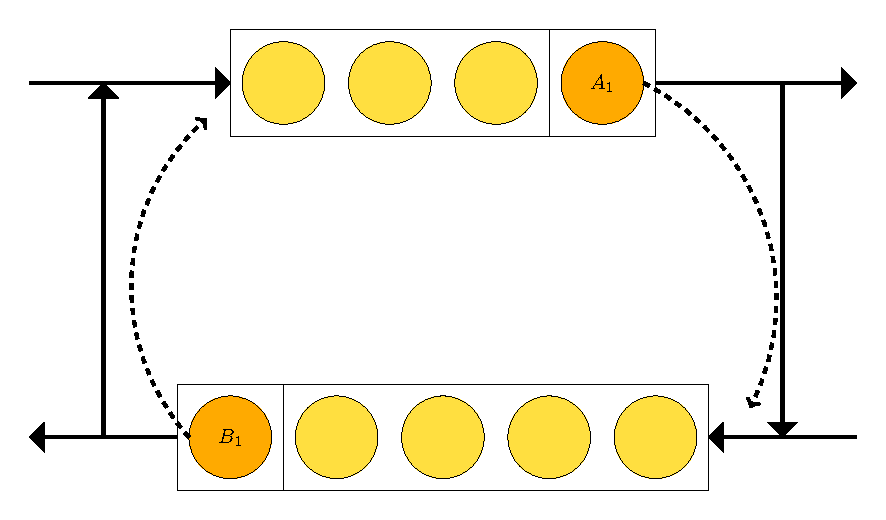
\includegraphics[width=0.8\textwidth]{../images/2nodesindeadlock.pdf}
\end{center}
\end{frame}

\begin{frame}
\begin{center}
\includestandalone[width=0.8\textwidth]{../images/motivatingexample}\\
\vspace{20mm}
\footnotesize{Osorio, C. \& Bierlaire, M. \textit{An analytic finite capacity queueing network model capturing the propogation of congestion and blocking.} European journal of operational research, 196(3):996–1007, 2009.}
\end{center}
\end{frame}

\begin{frame}
\begin{center}
\includestandalone[width=\textwidth]{../images/buildupdigraph}
\end{center}
\end{frame}

\begin{frame}
\begin{theorem}\label{thrm:knot}
A deadlocked state arises at time $t$ if and only if $D(t)$ contains a knot.
\end{theorem}

\begin{theorem}
For queueing networks:
\begin{enumerate}
  \item with one node
  \item with two nodes, each with two or fewer parallel servers
  \item with a finite amount of nodes, each with a single-server
\end{enumerate}
a deadlocked state arises if and only if there exists in $D(t)$ a
weakly connected component without a sink node.
\end{theorem}

\end{frame}

\begin{frame}[fragile]
\begin{minted}{python}
import ciw

N = ciw.create_network(
    Arrival_distributions=[['Exponential', 6.0]],
    Service_distributions=[['Exponential', 3.0]],
    Transition_matrices=[[0.5]],
    Number_of_servers=[3],
    Queue_capacities=[2]
)

ciw.seed(1)
Q = ciw.Simulation(N, deadlock_detector='StateDigraph')
Q.simulate_until_deadlock()
Q.times_to_deadlock
\end{minted}
\end{frame}


\begin{frame}
\begin{center}
\includestandalone[width=\textwidth]{../images/2nodemultiserver}
\end{center}
\end{frame}

\begin{frame}
    \frametitle{Times to Deadlock}
    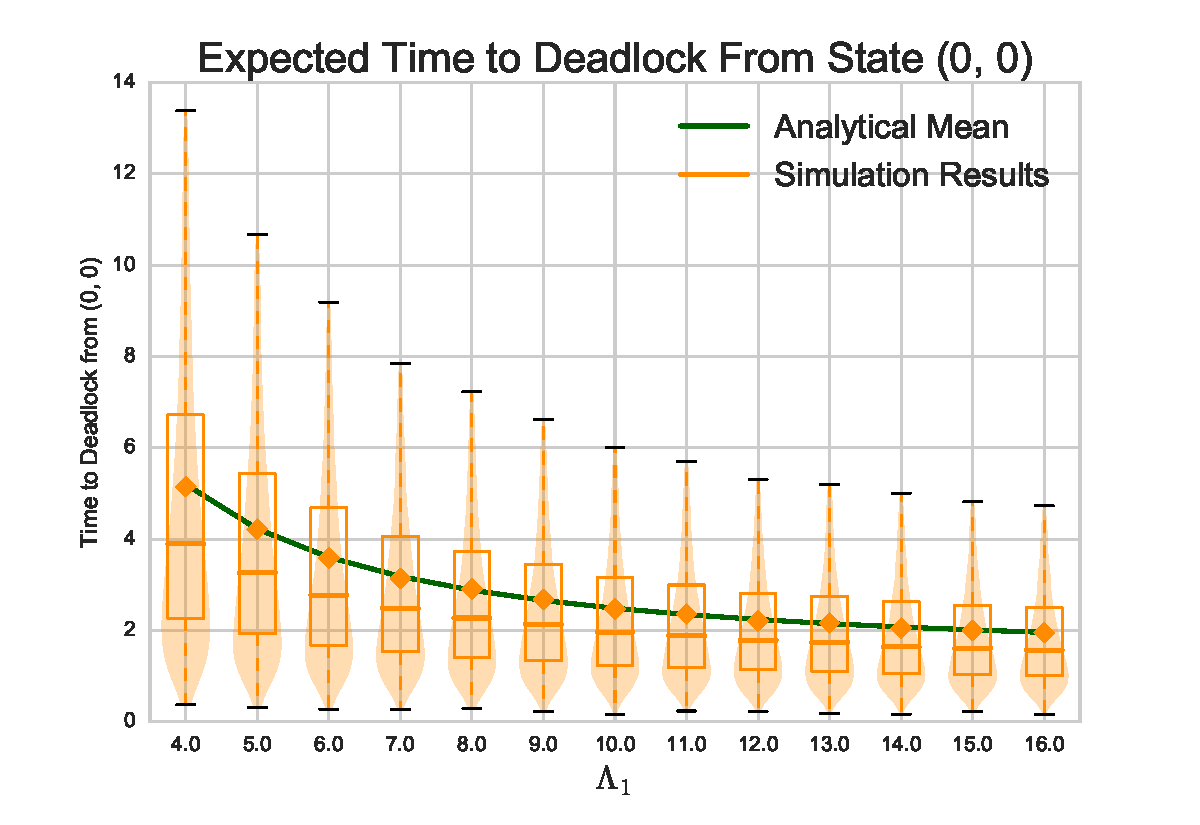
\includegraphics[width=0.5\textwidth]{../images/varyL1_2Nms}
    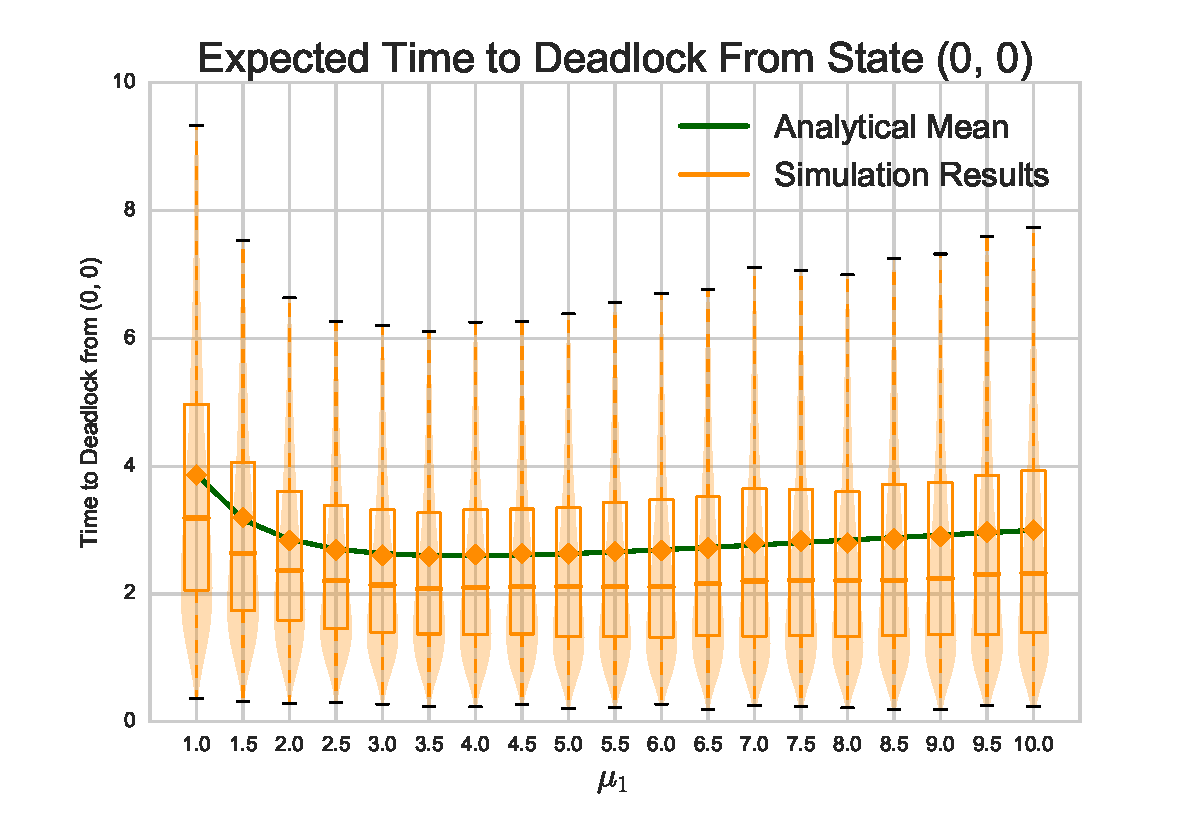
\includegraphics[width=0.5\textwidth]{../images/varymu1_2Nms}\newline
    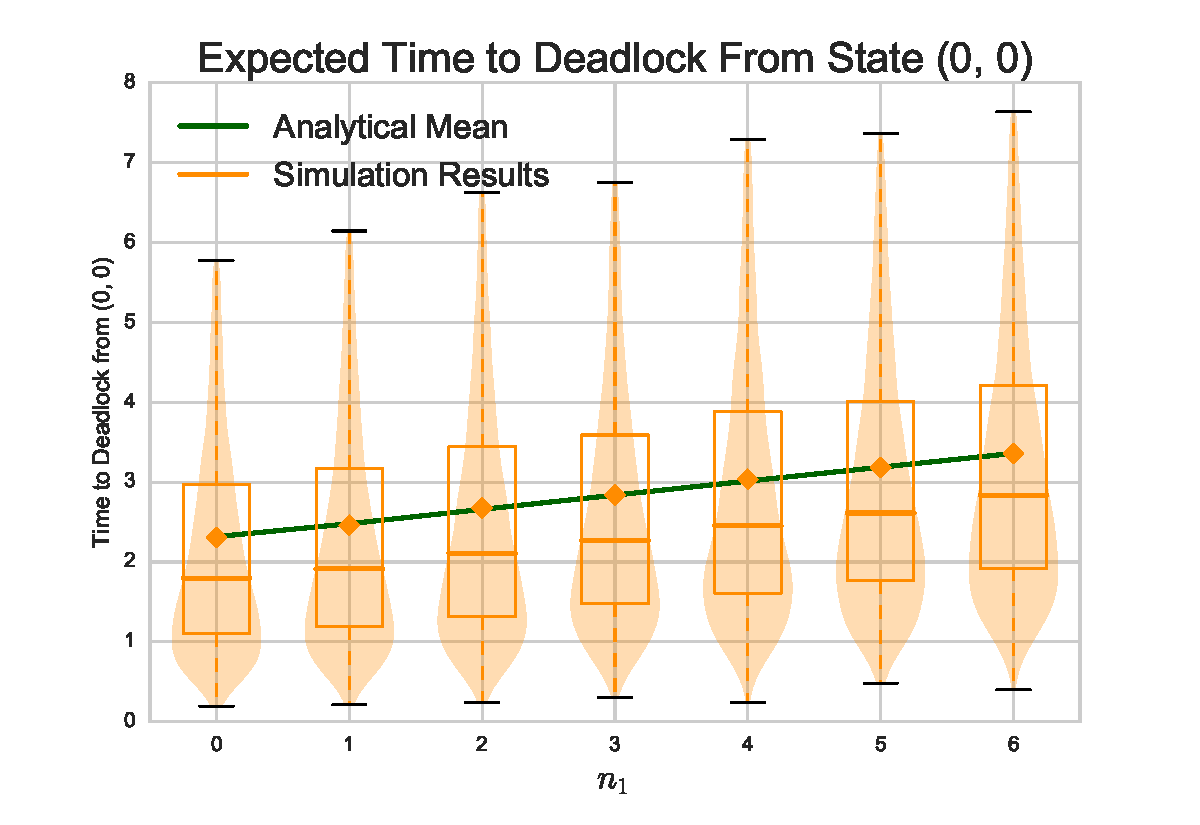
\includegraphics[width=0.5\textwidth]{../images/varyn1_2Nms}
    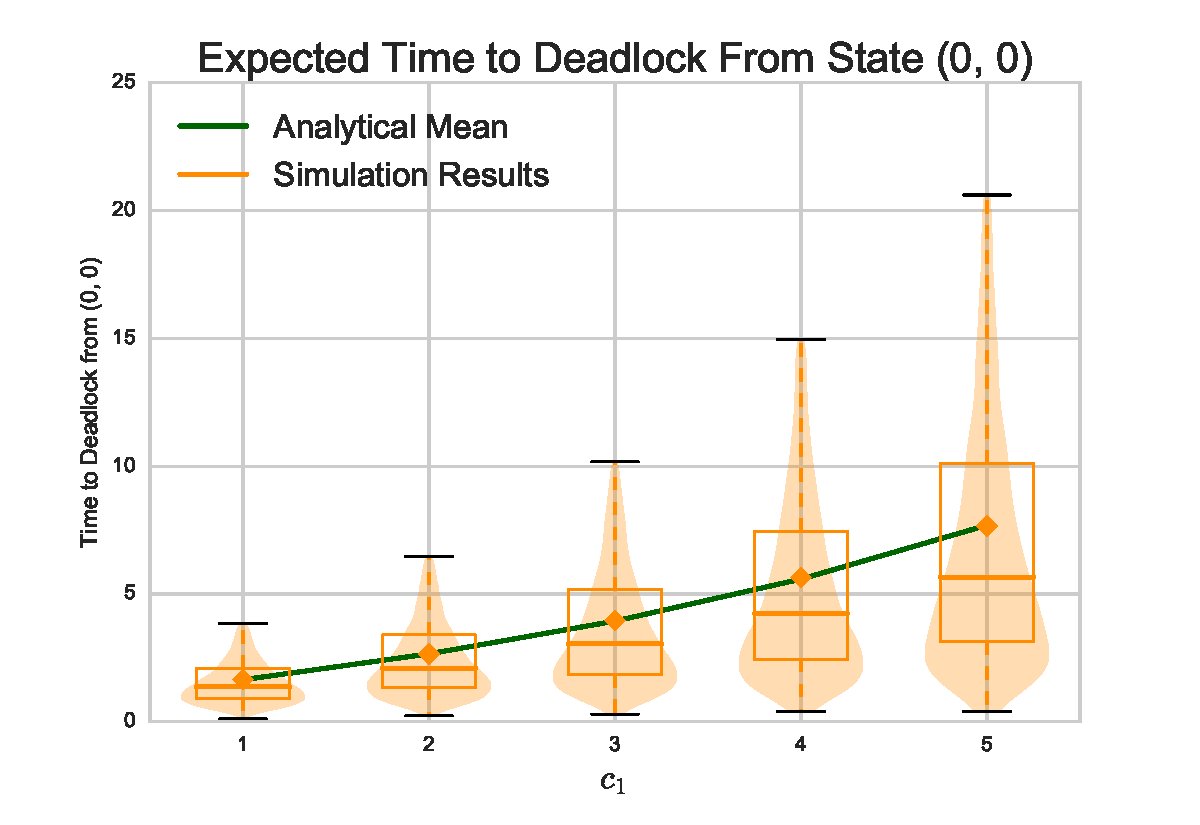
\includegraphics[width=0.5\textwidth]{../images/varyc1_2Nms}
\end{frame}

% \begin{frame}{Evaluating Newport Stay Well Plans}
% \begin{itemize}
% \item Risk stratification identifies individuals at risk of admission to institutionalised care or becoming frequent users of high cost care
% \item Develop holistic personal Stay Well Plans for these individuals, utilising low and no cost services
% \item Focused around pro-active patient centred coordinated care
% \item Aim to keep individuals and carers as well and as independent as possible
% \end{itemize}
% \end{frame}

\begin{frame}{Evaluating Newport Stay Well Plans}
\begin{itemize}
\item Risk stratification
\item Personal Stay Well Plans - low and no cost services
\item Pro-active patient centred coordinated care
\item As well and as independent as possible
\end{itemize}
\end{frame}

\begin{frame}
\begin{center}
\includestandalone[width=0.9\textwidth]{../images/swp_map}
\end{center}
\end{frame}

\end{document}
